\chapter{Use Cases and Supplemental UML Diagrams}

When starting a new software project, it is tempting to begin coding
immediately. An advocate of stepwise refinement starts with the
procedure \texttt{main()} that every program has, and grows the program
gradually by elaboration from that point. For complex systems, a
software designer should do more planning than this. Chapters 9 and 10
covered the basics of class diagramming, an activity that allows you to
plan out your data structures and their interrelationships.

The hard part about class diagramming is figuring out what information
will need to be stored in attributes, and what object behavior will
need to be implemented by methods. For many large projects there are
basic questions about what the program is supposed to do that must be
answered before these details about the application's
classes can be determined. In addition, class diagrams depict static
information but model nothing about the system that involves changes
over time.

This chapter discusses some UML diagramming techniques that are useful
before you start coding. They can help you figure out the details that
belong in your class diagrams, by modeling dynamic aspects of your
application's behavior. When you are finished with
this chapter you will know how to:

\begin{itemize}
\item Draw use case diagrams that show the relationships between
      different kinds of users and the tasks for which they will use the
      software.
\item Describe the details of use cases that define an application's tasks.
\item Draw statechart diagrams that depict an object's behavior as states and
      transitions between states that model the dynamic aspects of the
      application.
\item Specify conditions and activities that occur when an event causes an
      object to change its state.
\item Draw collaboration diagrams that illustrate dynamic interactions between
      groups of objects.
\end{itemize}


\section{Use Cases}

A \index{use case}\textit{use case} is an individual task. It defines a
unit of functionality that the software enables one or more users to
carry out. Sometimes it is a challenge to figure out what makes a
reasonable ``unit of functionality'' in an
application where long sequences of complex tasks are performed. Should
the use cases correspond to small units such as individual user actions
such as mouse clicks, or longer jobs such as updating a spreadsheet?
One way to identify the appropriate units of functionality is to ask,
for any given user action, whether it completes a change to the state
of the application data. If the user would likely want to be able to
save their work afterwards, the task is large enough to constitute a
use case.

A diagram showing all the use cases helps early on in development to
identify the overall \index{scope}scope and functionality of the
software system as seen from the outside. The components of a use case
diagram are depicted in Figure 13-1.

\bigskip

\begin{center}
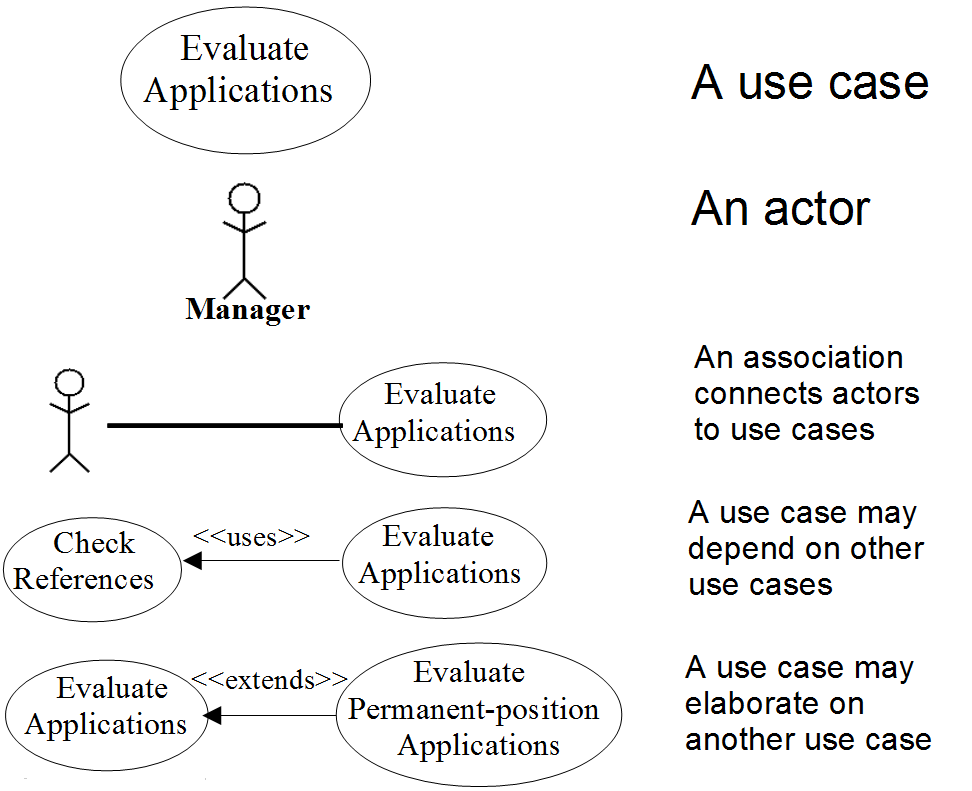
\includegraphics[width=5.0in,height=4in]{ub-img/usecase.png}

{\sffamily\bfseries Figure 13-1:}
{\sffamily The main components of use case diagrams}
\end{center}


The \textit{use cases} themselves are shown as ovals. The name of the
use case is inside the oval. The use cases have an accompanying
description; an example description is given in the next
section. A use case is not represented in software by a class, but
rather in the logic of the program's control flow. A
use case relates several otherwise unassociated objects for a limited
time to accomplish a particular task.

The term \index{actor}\textit{actor} denotes both human users and
external hardware or software systems that interact with the software
system under design. Actors are shown in use case diagrams as stick
figures. Each stick figure in the diagram represents a different kind
of actor that interacts with the system during one or more use cases.
The name of the \index{role}role is written under the stick figure. An
actor is really just a special kind of class that represents an
external, asynchronous entity.

The \index{association}\textit{associations} between use cases
and the actors that perform those tasks are drawn as plain lines. A use
case may be performed by one or several
actors. Use case associations identify the actors that participate in
each use case. They are only slightly related to the associations
between classes found in class diagrams.

\textit{Dependencies} and \index{elaboration}\textit{elaborations} between use
cases are drawn as lines with arrows, annotated with a label between
% \guillemotleft{ } and \guillemotright. Some use cases use other use cases as
{\textless\textless} and {\textgreater\textgreater}. Some use cases
use other use cases as
part of a more complex task. Other use cases are defined as extensions of
another use case.

\subsection*{Use case diagrams}

A use case diagram consists of a set of use case ovals, bordered by a rectangle
that signifies the extent of the software system. Actors are drawn outside the
rectangle, with connecting lines to those use cases in which they
participate. When some actors are non-human external systems, by convention the
human actors are depicted on the left, and the non-humans go on the right.

An example use case diagram is shown in Figure 13-2, which depicts a
recruiting management system. The manager hiring a new employee may
interact with the company's legal department to
produce an acceptable position advertisement. Many applicants might
apply for a given position. The manager evaluates applications,
possibly interviewing several candidates. When a candidate is selected,
the manager interacts with the legal department to make a job offer.

\begin{center}
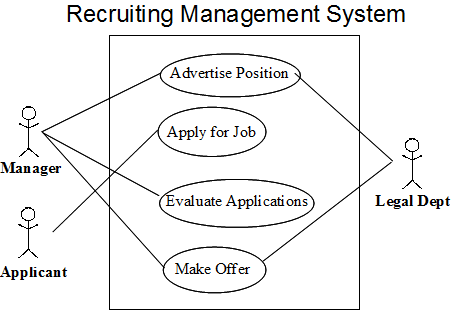
\includegraphics[width=4.5in,height=3.15in]{ub-img/usecase2.png}

{\sffamily\bfseries Figure 13-2}
{\sffamily A Use Case Diagram}
\end{center}

\subsection*{Use case descriptions}

The details of each use case are specified in a related \textit{use case
description}. This description may include prose text, such as the
following description of the ``Make Offer'' use case:

\textbf{Make Offer} is started by the manager when an applicant has been
selected from among the candidates for a position. The manager obtains
approval from the legal department, commits necessary budget resources,
and generates an offer letter with details on salary, benefits, and the
time frame in which a decision is required.

The use case description may be organized into fields, or more
detailed than this. For example, one field might consist of the
most common sequence of events, emphasized by an explicit enumeration.
The common variations on the primary event sequence are also of
value. A more organized description of the Make Offer use case might
be

\paragraph[Make Offer]{\bfseries Make Offer}
\textbf{Initiated}: by manager, after candidate for a position has been
selected.

\textbf{Terminates}: when the candidate receives the offer in writing.

Sequence:

1.\ \ Manager obtains approval from legal department.

2.\ \ Manager commits resources from budget

3.\ \ Manager telephones candidate with offer

4.\ \ Manager generates offer letter

5.\ \ Offer letter is express mailed to candidate.

Alternatives:

In step 2, Manager may request extra non-budgeted resources.

In step 3, Manager may fax or e-mail offer in lieu of telephone.

\section{Statechart Diagrams}

\index{statechart}\textit{Statecharts} are diagrams that depict finite
state machines. A \index{finite state machine}finite state machine is a
set of states, drawn as circles or ovals, plus a set of transitions,
drawn as lines that connect states. Statecharts generally have an
\textit{initial state}, which may be specially designated by a small,
solid circle, and one or more \textit{final states}, which are marked
by double rings.

In object modeling, states represent the values of one or more
attributes within an object. Transitions define the circumstances or
events that cause one state to change to another. Statecharts are a
tool for describing allowable sequences of user interactions more
precisely than is captured by use cases. Discovering the events that
cause transitions between states, as well as the conditions and actions
associated with them, helps the software designer to define the
required set of operations for classes.

Figure 13-3 shows an example statechart diagram for a real estate
application. A house enters the FORSALE state when a listing agreement
is signed. The house could leave the FORSALE state with a successful
offer at the listed price (entering a REVIEW period) or by utter
failure (if the listing agreement expires), but the most common
occurrence is for a buyer to make an offer that is less than the asking
price. In that case, a NEGOTIATION state is entered, which may iterate
indefinitely, terminating when either the buyer or seller agrees to the
other party's offer or walks away from the discussion.
When an offer is accepted, a PENDING period is entered in which
financing is arranged and inspections and walkthroughs are performed;
this period is terminated when escrow is closed, title is transferred,
and the house is SOLD.


\bigskip

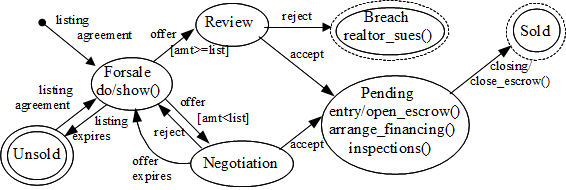
\includegraphics[width=5.8in,height=2.0in]{ub-img/statechart.png}

{\sffamily\bfseries Figure 13-3:}
{\sffamily A Statechart Diagram}

\bigskip

Since a state represents the values of one or more attributes within an
object, a transition coincides with assignments that alter those
attributes' values. The purpose of the diagram is to
identify when and why those values change, in terms of the application
domain.

\subsection*{Events and conditions}

Most transitions in a statechart are triggered by an \index{event,
  statechart}\textit{event}. In Figure 13-3 the events were things like
``offer'' and ``closing''.  Typically, an event describes an asynchronous
communication received from another object. An event is instantaneous, while a
state corresponds to some possibly lengthy interval of time until an object
transitions into some other state.  From the point of view of the object being
modeled in the statechart, the event is an interrupt that affects the object's
behavior. Such an event would normally be implemented by defining a method for
the object with a name derived from the event name.

It is common during modeling to have a transition that can only occur if a
Boolean condition is satisfied. In Figure 13-3, the event offer was used for
two transitions out of the same state, with different conditions (amount
{\textgreater}= list price versus amount {\textless} list price) to determine
which transition would be taken. In statechart diagrams, conditions are given
after the event name, in square brackets, as in
\texttt{[amt {\textless} list]}.

For a condition on a transition, it might make sense for that
transition to require no trigger event at all. The transition would
occur immediately if the condition were ever satisfied. Such a
constraint-based transition would potentially introduce condition tests
at every point in the object's code where the
condition could become true, such as after each assignment to a
variable referenced in the condition. This may work in special
cases, but poses efficiency problems in general. Transitions without
trigger events make sense in one other situation. If a state exits when
a particular computation completes, you can use a triggerless
transition to the new state that the object will be in when it is
finished with the job it is performing in the current state.

\subsection*{Actions and activities}

Events are not the only class methods that are commonly introduced in
statecharts. In addition to a condition, each event can have an
associated \index{action, statechart}\textit{action}. An action is a
method that is called when the event occurs. Since events are
instantaneous, action methods should be of bounded duration.
Similarly, states can have a whole regalia of related methods called
\index{activity, statechart}\textit{activities}. There are activities
that are called when a state is entered or exited, respectively. The
most common type of activity is a method that executes continuously as
long as the object is in that state. If more than one such activity is
present, the object has internal concurrency within that particular
state.

In statechart diagrams, actions are indicated by appending a slash (/)
and an action after the event name and any
condition. Activities are listed within the state
oval. If a keyword and a slash prefix the activity, special semantics
are indicated. For example, the \texttt{do} keyword indicates
repeated activity. In Figure 13-3, the activity
\texttt{do / show()} says that the house will be shown repeatedly
while it is in the FORSALE state. The activity \texttt{entry /
open\_escrow()} indicates that the method \texttt{open\_escrow()} is
called on entry to the PENDING state, after which
\texttt{inspections()} and \texttt{arrange\_financing()} activities are
performed.

\section{Collaboration Diagrams}

Statecharts normally model the state of one
object. They show how the object reacts to events that come from the
other objects in the system, but do not depict where those events came
from. In a complex system, it is useful to understand
the interactions among many objects. An event that changes one
object's state may trigger events in many other
objects, or a group of objects may trigger events in one another in a
cyclic fashion.

\index{collaboration diagram}\textit{Collaboration diagrams} show such
interactions between objects. They are drawn similarly to class diagrams. A
group of rectangles are drawn to represent \index{instance!class}instances of
classes, and lines depict the relationships between those classes. But while a
class diagram emphasizes the static structures, representing details such as
class attributes, and association multiplicity, a collaboration diagram depicts
a specific sequence of messages sent from object to object during the
completion of some task. The messages are annotated alongside the
links between objects to indicate sender and recipient, and numbered
to show both the sequence and the \index{tree}tree structure of the
nested messages. In the general case more than
one message number can be annotated for a given \index{link!association
  instance}link, since multiple messages may be transmitted between the same
objects in the course of completing the use case.

Figure 13-4 shows an example collaboration diagram. This particular
collaboration illustrates the input processing of a user event in a game
application in which pieces are moved about a board, such as chess or
checkers. The incoming event is sent as a message from the window object to the
board widget (message 1). The board widget uses its layout to map mouse (x, y)
coordinates onto a particular square to which the user is moving the currently
selected piece, and forwards a message to that square (1.1). The square sends a
message to a rules object, which checks the validity of the user's move
(1.1.1), and if the move is legal, the square sends a message to the
game piece, effectively telling it to move itself (1.1.2). The game
piece sends an ``erase''
message to the square where it was formerly located (1.1.2.1) before changing
its link to refer to the square to which it is moving.

\bigskip

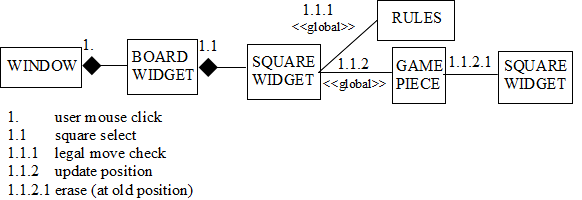
\includegraphics[width=5.5in,height=2.1in]{ub-img/collabor.png}

{\sffamily\bfseries Figure 13-4:}
{\sffamily A Collaboration Diagram}

\bigskip

There are a couple more annotations worth noting in Figure 13-4. The links
between window, board widget, and square widget are identified as aggregations
since they denote geometric containment; this information is redundant with the
class diagram, but is given to explain how the objects are linked to allow
message transmission. The connections between the square widget and the rules
and game piece objects are marked as
{\textless}{\textless}global{\textgreater}{\textgreater} to indicate that the
square widget obtains references to these objects from global variables. The
link between the game piece and the square widget in which it is located is a
regular association and does not require further annotation. Besides
{\textless}{\textless}global{\textgreater}{\textgreater} you can annotate a
link as a {\textless}{\textless}parameter{\textgreater}{\textgreater} or
{\textless}{\textless}local{\textgreater}{\textgreater} to indicate other
non-association references through which messages are transmitted.

\section{Summary}

This chapter introduced four UML diagram types that
are useful in modeling dynamic aspects of a program's behavior. To
learn more about these techniques and others, consult
a primary UML resource, such as
\textit{The Unified Modeling Language User Guide}, by
Grady Booch, James Rumbaugh, and Ivar Jacobson.

No one technique is a complete solution, but some combination of use
cases, statecharts, and collaboration diagrams will allow you to
sufficiently model most applications. Use cases are particularly
valuable for describing tasks from the point of view of the
application domain and human user. Statecharts are good for modeling
event-based systems such as user interfaces or distributed network
applications.  Collaboration diagrams describe interactions between
objects that allow you to model the big picture in a complex system.

In terms of primacy and chronological order, for most applications you should
start with use cases and try to develop them completely. For those use cases
that seem complex, or for which the conventional use case description seems
inadequate, you can then bring in statecharts or collaboration diagrams to
assist in completing an understandable design.

Class diagrams are the backbone of a detailed object oriented design.  They can
be developed by extracting details from the other kinds of diagrams, and should
reflect programmers' understanding of the application domain for which the
software is being written.
